\documentclass[11]{report}
\usepackage{graphicx}
\usepackage[a4paper]{geometry}
\usepackage{amsmath}
\usepackage{amssymb}
\usepackage{float}
\usepackage[utf8]{inputenc}
\usepackage[english]{babel}


\renewcommand{\baselinestretch}{1.2}
\geometry{margin=1in}
\pagenumbering{arabic}
\pagestyle{plain}
\begin{document}
\begin{titlepage}
\begin{center}
\vspace*{1cm}
\LARGE
\textbf{Documentation for Differential Forms Summer Project}\\
\vspace{5cm}
\normalsize
\textbf{Moustafa Gharamti, Samuel Kirwin-Jones, Maciej Tomasz Jarema}\\

\end{center}
\end{titlepage}

\section{Geometry of stack vectors}

\subsection{Translations needed to define stack vectors and arrowheads}
Stack vectors are covariant vectors, defined by planar sheets (lines, when working in 2D) perpendicular to arrows of the contravariant vector. The density of these planes, is determined by magnitude of the vector field at each point in space. These stack vectors, being covariant, correspond to differential forms, while arrow vectors (being contravariant) correspond to vector fields.\\
In python, these stack sheets have to be defined from the magnitude and direction of the input, based on \(x\) and \(y\) components of the 1-from.

\begin{figure}[H]
	\centering
	%\graphicspath{ {c:/Users/macus/Desktop/Uni/summer internships/Moustafa - Differential Forms/images/} }
	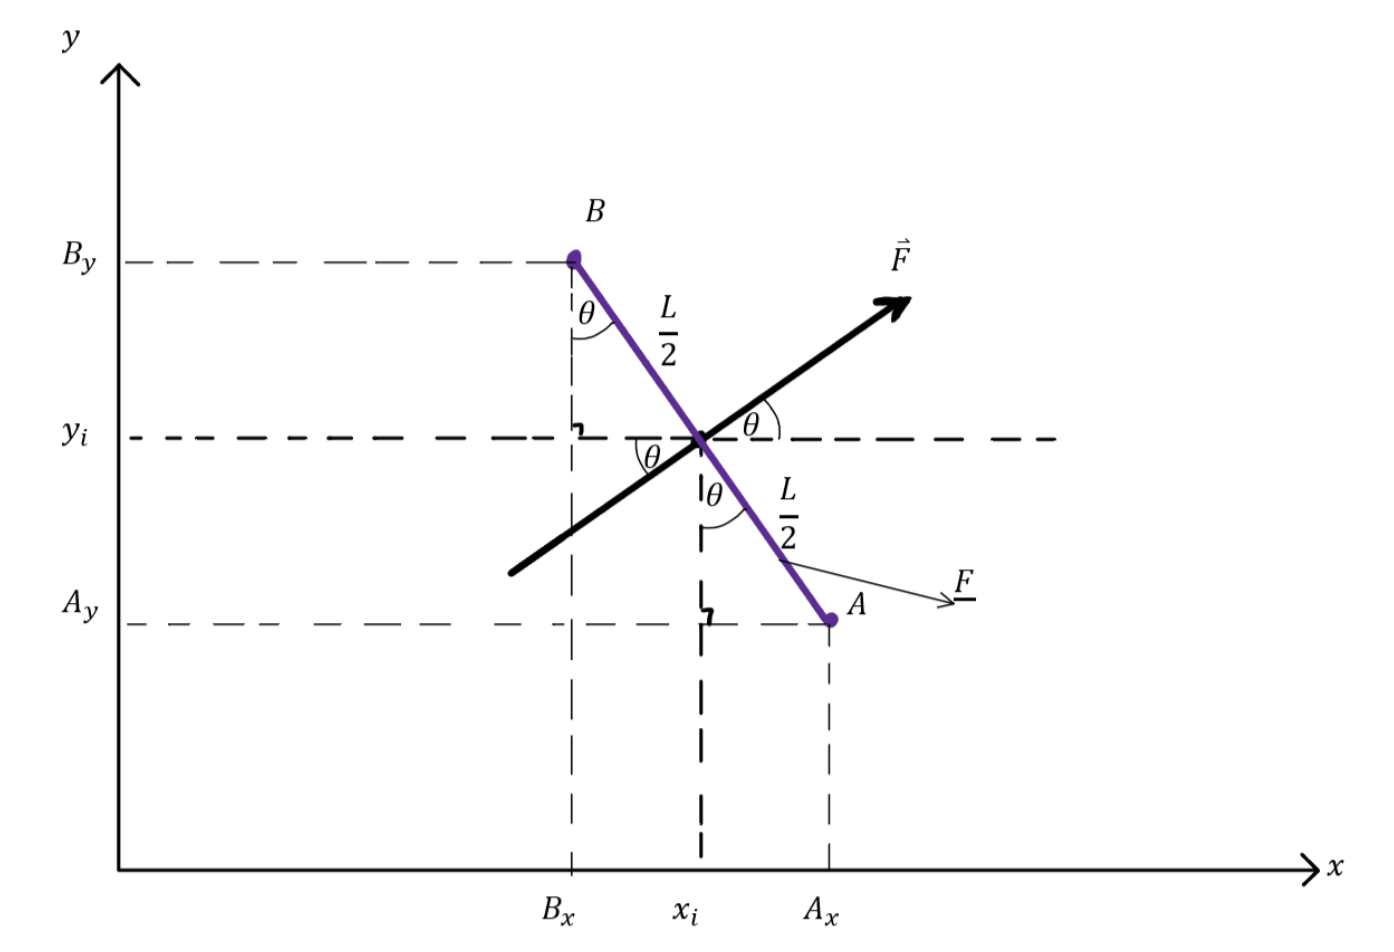
\includegraphics[scale=0.4]{Documentation_images/Geometry of 1 stack sheet}
	\caption{Sketch presenting the Geometrical arguments needed to define stack sheets, based on field magnitude and direction(indicated well by an arrow vector as shown)}
	\label{fig:1 sheet}
\end{figure}
\noindent For \( x_i\) and \( y_i\) marking the $i$\textsuperscript{th}  considered position in the field, with its corresponding angle to the $x$-axis (ccw). Technically, points \(A\) and \(B\) as well as $\theta$ and $\vec F$ depend on the position in space that is considered, therefore, should include the subscript, '\(i \)'. This was not added for figure clarity. \\
The stack, shown in purple, is perpendicular to $\vec F$  with end points $A$ and $B$ separated by distance $L$ (in the code, defined as a fraction of graph scale).\\
From these, through simple geometry, one obtains the following equations:
\begin{equation}
\label{T1} \begin{split}
A_x &= x + \left( \frac{L}{2} \right) \sin( \theta)\,,\\
A_y &= y - \left( \frac{L}{2} \right) \cos( \theta)\,,\\
B_x &= x - \left( \frac{L}{2} \right) \sin( \theta)\,,\\
B_y &= y + \left( \frac{L}{2} \right) \cos( \theta)\,,
\end{split}
\end{equation}
describing the positions of points \(A\) and \(B\) in terms of their Cartesian components.\\
These also function generally as operations that displace a point on the vector in the direction perpendicular to the arrow, by a corresponding length - here by \( \frac{L}{2} \)\,. \\

To then displace the stack sheet by distance $d$ in the direction parallel to the arrow as shown in Figure~\ref{fig:parallel disp.},
\begin{figure}[H]
	\centering
	%\graphicspath{ {c:/Users/macus/Desktop/Uni/summer internships/Moustafa - Differential Forms/images/} }
	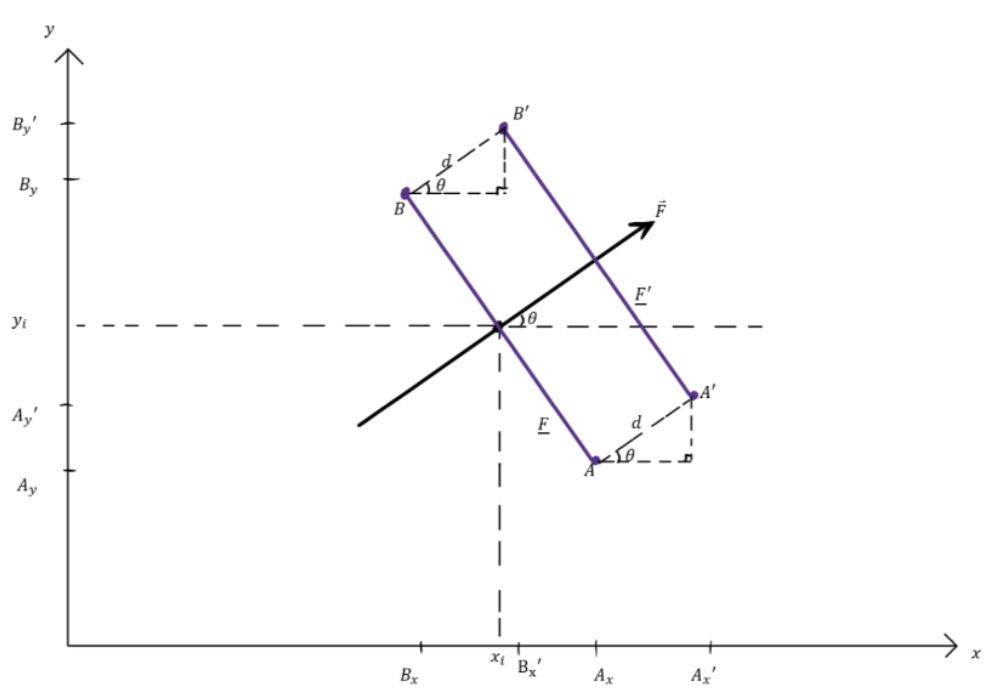
\includegraphics[scale=0.38]{Documentation_images/Geometry of 1 stack sheet, displacement 1}
	\caption{Sketch presenting the geometrical arguments needed to displace stack sheets in the direction parallel to the vector field direction at that point, (again - represented by an arrow)}
	\label{fig:parallel disp.}
\end{figure}
\noindent we use the following translation equations:
\begin{equation}
\label{T2} \begin{split}
A_x' &= A_x + d \cos(\theta)\,, \\
A_y' &= A_y + d \sin(\theta)\,, \\
B_x' &= B_x + d \cos(\theta)\,, \\
B_y' &= B_y + d \sin(\theta)\,, 
\end{split}
\end{equation}
which again function as general operations for such parallel displacements by any distance \( d \), from the centre.\\
To define the arrowhead on that stack vector, both translation operations, eqs. (\ref{T1}, \ref{T2}), need to be used to obatin points to be connected as shown on the figure below

\begin{figure}[H]
	\centering
	%\graphicspath{ {c:/Users/macus/Desktop/Uni/summer internships/Moustafa - Differential Forms/images/} }
	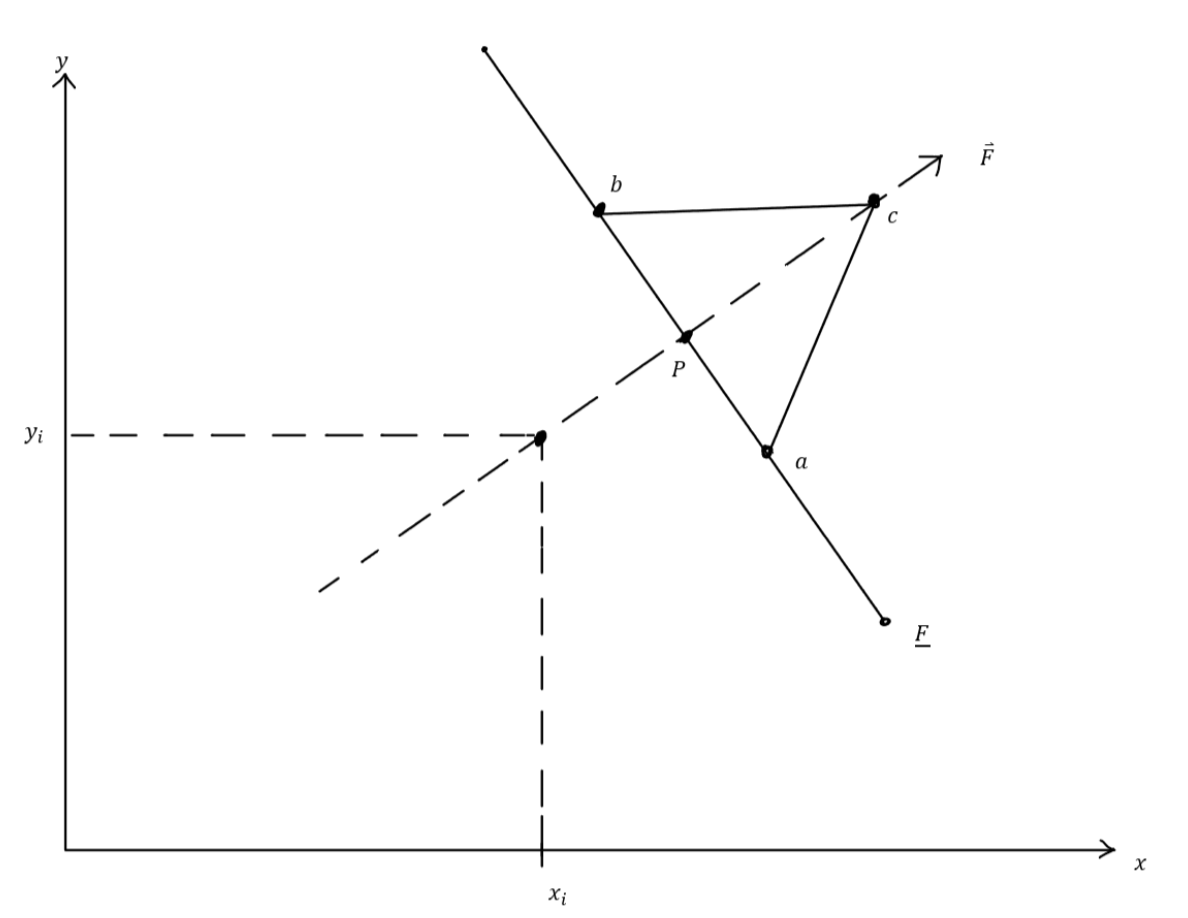
\includegraphics[scale=0.3]{Documentation_images/Geometry of 1 stack sheet, displacement 2}
	\caption{Sketch presenting the geometrical arguments needed to define the arrowhead on each stack vector)}
	\label{fig:arrowhead gometry}
\end{figure}
\begin{align*}
P_i &= \left( x_i + \frac{L_s}{2} \cos( \theta_i) , \  y_i + \frac{L_s}{2} \sin( \theta_i) \right) \\
a_i &= \left( P_{x, i} + \frac{L_s}{w_{head}} \sin( \theta_i) , \  P_{y, i} - \frac{L_s}{w_{head}} \cos( \theta_i) \right)\\
b_i &= \left( P_{x, i} - \frac{L_s}{w_{head}} \sin( \theta_i) , \  P_{y, i} + \frac{L_s}{w_{head}} \cos( \theta_i) \right)\\ 
c_i &= \left( x_i + \frac{L_s}{h_{head}} \cos( \theta_i) , \  y_i + \frac{L_s}{h_{head}} \sin( \theta_i) \right)
\end{align*}
\noindent In these equations, variables are defined as shown on the above figure. \( L_s \) is the maximum thickness of the stack, parallel to the direction of the considered vector field, \( w_{head} \) is the width of the base of the arrowhead that rests on the last stack, and \( h_{head} \) is the height of the arrowhead parallel to the vector field direction.

Note that each has also been assigned a subscript \( i \) which does not appear on the figure. This is only done as these coordinates depend on the point in space that is currently being considered. Also note, that for a single sheet in the stack, the initial displacement from \( (x, \ y )\) to \( P \) must be omitted.

\subsection{General from of stack sheet positions, for any number of sheets}

In the code, it was important to define the displacements of each stack sheet, form the middle position of the arrow vector, at each point in the field. Positioning of sheets depends on the magnitude of the vector field at that point in space. The larger the magnitude, the higher the sheet density. As the spread of the sheets is limited to a pre-defined maximum (on the plot, not physically), this increase in density corresponds to more stack sheets being present.\\
One way of plotting these, such that all sheets are equally-spaced is to consider odd and even number of stacks separately. We define them by displacing stack sheets along the arrow by certain lengths (as per the equations above) from the middle position (the considered position in the field).\\

\noindent For {\bf odd number of stack sheets}, the following pattern was noticed:\\
\small
For 1 sheet: no displacing is needed $\Rightarrow$ $\pm0$\\
For 3 sheets: none, and ends of the stack $\Rightarrow$ $\pm0$ and  $\pm\frac{1}{2}$ $\longrightarrow$ technically $\pm\frac{1}{2}$ $\cdot$ $L_s$\\
For 5 sheets: none, ends, and points equally between $\Rightarrow$ $\pm0$, $\pm\frac{1}{2}$ and $\pm\frac{1}{4}$\\
For 7 sheets: $\Rightarrow$ $\pm0$, $\pm\frac{1}{2}$, $\pm\frac{2}{6}$ and $\pm\frac{1}{6}$ $\longrightarrow$ At this point, note that $\frac{3}{6} = \frac{1}{2}$ (obvious but important)\\
For 9 sheets: $\Rightarrow$ $\pm0$, $\pm\frac{1}{2}$, $\pm\frac{3}{8}$, $\pm\frac{1}{4}$ and $\pm\frac{1}{8}$ $\longrightarrow$ Again, $\frac{1}{4} = \frac{2}{8}$ and $\frac{1}{2} = \frac{4}{8}$\\
For 11 sheets: $\Rightarrow$ $\pm0$, $\pm\frac{1}{2}$, $\pm\frac{4}{10}$, $\pm\frac{3}{10}$, $\pm\frac{2}{10}$  and $\pm\frac{1}{10}$\\
\vdots\\
\normalsize
\noindent These display the following recursion:\\
The displacement along the arrow as a fraction of total stack length $L_s$, of the $s$\textsuperscript{th} sheet, when drawing $n$ stack sheets overall, for odd $n$ is:

\[ \pm{ \frac{s}{ \left( n-1 \right) }}\,, \]

\noindent where we require the fractional displacement (from the middle position) to not exceed half of the total length therefore:\\
\[ 1 < s < \frac{1}{2} \left( n-1 \right)\,.\]\\

\noindent For {\bf even number of stack sheets} this pattern emerges:\\
\small
2 sheets:$\Rightarrow$ $\pm\frac{1}{2}$\\
4 sheets:$\Rightarrow$ $\pm\frac{1}{2}$ and $\pm\frac{1}{6}$\\
6 sheets:$\Rightarrow$ $\pm\frac{1}{2}$, $\pm\frac{3}{10}$ and $\pm\frac{1}{10}$ $\longrightarrow$ Note again that $\frac{1}{2} = \frac{5}{10}$.\\ From here on continue with those not reduced fractions:\\
8 sheets: $\Rightarrow$ $\pm\frac{1}{14}$, $\pm\frac{3}{14}$, $\pm\frac{5}{14}$ and $\pm\frac{7}{14}$\\
10 sheets:  $\Rightarrow$ $\pm\frac{1}{18}$, $\pm\frac{3}{18}$, $\pm\frac{5}{18}$, $\pm\frac{7}{18}$ and $\pm\frac{9}{18}$\\
\vdots\\
\normalsize
These display the following recursion:\\
The displacement along the arrow as a fraction of total stack length of the $s$\textsuperscript{th} sheet, when drawing $n$ stack sheets overall, for even $n$ is:

\[ \pm\frac{2s+1}{2 \left( n-1 \right) }\,, \]

\noindent where we require the fractional displacement to not exceed half of the total length therefore:

\[ 1 < s < \frac{1}{2} \left( n-2 \right)\,. \]

\noindent Alternatively, each can be defined separately, manually, if a small amount of sheets is needed.

\subsection{variables in stack plot code}

This has been implemented in code. The parameters for this are as follows:

\begin{itemize}
	\item $L$ is the length of the positive $x$ and $y$ axes,
	\item pt\textunderscore den is the number of points along each axis,
	\item $a$ is a linear scaling of the field,	
	\item $u$ is the vector field $x-$component, $v$ is the vector field $y-$component $\longrightarrow$  Alternatively: $Fr$ is the radial component and $Ftheta$ is the angular component
	\item orientation is a sting that defines how the arrows pivot,
	\item scale is a linear scale on the quiver plot arrows,
	\item delta is the extra length along the axis to show, past the defined grid, full emerging arrows from border points,
	\item fract is the fraction of graph length equal to stack sheet in direction perpendicular to arrow,
	\item s\textunderscore max is the maximum number of stacks to use,
	\item sheet\textunderscore L is the length of stack perp. to arrow,
	\item s\textunderscore L is the maximum length of stack sheet parallel to arrow,
	\item w\textunderscore head is the width of the arrowhead base as the fraction of the stack sheet length perpendicular to the arrow,
	\item h\textunderscore head is the length of the arrowhead parallel to the arrow, as the fraction of the total stack size parallel to the arrow,

\end{itemize}


\section{Initial GUI of the quiver and stack plot}

\subsection{Explaining user defined functions in the GUI code}

\textbf{parity}: this function takes an input of an integer and returns True ($1$) is it is even and False ($0$) when it is odd. It is useful when defining stack sheets as displacements from the middle position, as the formulas are different for even and odd number of sheets per stack.\\
\textbf{G}: it takes three inputs $\Rightarrow$ $s$: the recursion of sheet displacing from the middle position (which pair is being completed), $n$: how many sheets are to plotted in total and $c$: which is the \textbf{bool} value from the parity function\\
\textbf{stack\textunderscore plot}: takes the following inputs:
\begin{itemize}
	\item $xg$ and $yg$: the grid of points to be used when plotting the field
	\item $ax$: the axis to plot on
	\item $u$ and $v$: the $x-$ and $y-$components of the vector field to be plotted
	\item s\textunderscore max: maximum number of sheets to plot, changes how dense the plot appears
	\item $L$: changes the size of axis (in both x and y equally, from origin)
	\item pt\textunderscore den: defines the number of points on each axis that create the grid
	\item fract: defines the size of the stack sheet (as a square) as a fraction of total graph size
	\item arrows (optional, default=True): Bool variable, defines if arrows should be plotted on top of the stacks (when True), or if only stacks are to be plotted (when False)
	\item orientation (optional, default='mid'): sets the pivoting point of the arrows about that grid point that they are defined at.
	\item scale (optional, default=1): Linearly scales the arrows in the quiver plot
	\item w\textunderscore head (optional, default=8): sets the fraction that defines the width of the arrowhead at its base (on the stack), from the total size of the stack.
	\item h\textunderscore head (optional, default=4): Sets the fraction that defines the height of the arrowhead parallel to the vector field magnitude at that point, from the total size of the stack.
\end{itemize}
\textbf{on\textunderscore key\textunderscore press}: Function that tracks mouse key presses, needed for the 'Matplotlib' toolbar to function\\
\textbf{format\textunderscore eq}: Takes a single string, converts all variables in it that are common in vector field equations, and turns them into things that python can understand. Returns the corrected string\\
\textbf{eq\textunderscore to\textunderscore comps}: Takes the two strings given by the user (equations for the field in the $x$ and $y$ directions) as well as the x and y grids, and the previous (or initial arrays for) $u$ and $v$. Uses the above function (format\textunderscore eq) to make the string 'python readable'. If one or more of the strings is zero, it defines a zero array for the component to be zero over all points along the grid and for shapes to match. Otherwise, it evaluates the given equation and returns the vector field components $u$ and $v$\\
\textbf{vect\textunderscore type\textunderscore response}: Responds to changes in Radio-buttons that set the type of field to be plotted (arrow, stacks or both). Takes in a value from the Radio-buttons corresponding to the chosen field type. It clear the current plot. Checks which button has been selected and uses ax.quiver and previously user defined stack\textunderscore plot to create the updated graph. It then updates it on the GUI by using canvas.draw() for the canvas being defined on the main window, in its own frame. Returns no variables.\\
\textbf{PLOT\textunderscore response}: Responds to the 'PLOT' button being pressed. Updates the axis scaling, point density, maximum number of sheets per stack, linear scaling (`$a$') and the new field components. Takes in no input. collects all needed variables by the `.get()' method of Tkinter objects. After running, it plots the new specified field, with the new parameters as a stack only plot and changes the status of the Radio-buttons to one again be - stacks only (therefore for tensor (same variable name as in VFA java code) to equal 0)\\
\textbf{custom\textunderscore btn\textunderscore response}: when the button called `customise' is pressed, this function responds by opening a new (`optimisation settings') window, in which features can be customised. It includes entry boxes where the user can input new values for parameters such as `fract', `w\textunderscore head' and `h\textunderscore head' (described previously). These are initially filled with current values, changing them and pressing `SUBMIT ALL' updates the plot.\\
\textbf{custom\textunderscore submission}: Responds to the `SUBMIT ALL' in the new `optimisation settings' window. When the button is pressed, the input values are globally saved. The current axis are cleared, a new plot is constructed as per the new specifications and it is displayed on the `canvas' of the correct frame. The updated plot is initially only a stack plot, therefore the radio-buttons are returned to the original position of `stacks'. The new window is then closed.

\section{2-forms from 1-forms, exterior derivative (on $\mathbb{R}^{m}$)}
The code includes a script that calculates 2-forms from a given 1-form in a specified number of dimensions.
It requires input of the 1-form components respectively to their elemental 1-form (in code: string\textunderscore x, string\textunderscore y, etc.), variable arrays (in code: $x$, $y$ etc.) as well as grids (in code: $xg$, $yg$, etc.) of these and a list of symbols for each variable used in the equations (coords).
The code, so far, has to be changed manually to include the change of all given components from \textbf{string} type to \textbf{sympy.core.mul.Mul}. The number of used dimensions has to also be input as an integer ('$m$' in the code). The variable, 'expressions' has to also be appended with the correct number of components.

\noindent Python cycles over the components and the given symbols for variables, differentiating each. To improve efficiency, the derivatives have not been completed when components are to be differentiated with respect to their corresponding elementary 1-form (these go to zero). The results are saved into an (m $\times$ m) array called ext\textunderscore ds'. The array is of data type 'object', as it must store strings of arbitrary length in each of its components. It stores all the found derivatives, with components changing along the rows, and variables changing along the columns.
Each derivative expression is also changed into a string, This is done to append needed prefixes onto them and to later use them with the eval() function, such as brackets and negatives. Minus sings (strings) are then appended to the upper right hand-side of the matrix. This is done to correct for the elementary 2-forms being in the wrong order.

\noindent This, completed, array is then taken through loops that extract the components of each elementary 2-form. These components are symmetrical elements, therefore extracting them includes taking elements with the same $i$ and $j$, switched in the coordinates. A 'pair' variable is introduced to keep track of how many times the loop extracted a pair of 2-form components and merged them. As only 2-forms are being calculated, there is always 2 components being extracted toward one elementary 2 form (including zeros as components) The number that this variable reaches is the number of components of a 2 form on $\mathbb{R}^{m}$, which was found to be given by triangular numbers. Resulting pairs are stored in an array of 1 column and a number of rows determined  by the triangular number of dimensionality. This array is called 'result', and stores objects (it must consist of strings of varying lengths for each element). Each time a new pair is being considered, the element from 'result' is cleared to exclude the initial 'NoneType' variable present. When appending the components, it is checked that if one or more of them evaluated to zero, they are not appended.
The result is printed, as a vector, whose rows correspond to different 2-form elements. The order is as follows:
For m=3:
\begin{center}
	\begin{tabular}{c}
		$ dx \wedge dy$, 
		$ dx \wedge dz$, 
		$ dy \wedge dz$.
	\end{tabular}
\end{center}

For m=4 these become:

\begin{center}
	\begin{tabular}{c}
		$ dx \wedge dy$,
		$ dx \wedge dz$,
		$ dy \wedge dz$,
		$ dx \wedge dw$,
		$ dy \wedge dw$,
		$ dz \wedge dw$,
		
	\end{tabular}
\end{center}
etc.

These follow the component pairs as they appear in the lower-right of the matrix (ext\textunderscore ds), in order that follows each line, until the main diagonal.
It can be clearly visualised on the example of the 2-form on $\mathbb{R}^{4}$ as follows:
\begin{equation}
		\begin{pmatrix}
			0 & dy \wedge dx & dz \wedge dx & dw \wedge dx \\
			dx \wedge dy & 0 & dz \wedge dy & dw \wedge dy \\
			dx \wedge dz & dy \wedge dz & 0 & dw \wedge dz \\
			dx \wedge dw & dy \wedge dw & dz \wedge dw & 0 \\
		\end{pmatrix}
\end{equation}

Each component of the outcome ('result') is then formatted in such a way as to be understood by python's eval() function and the evaluation of each is saved into a variable called 'form\textunderscore 2'. This has to be composed of m dimensional arrays, one for each elemental 2-form component (given by the triangular numbers from the used dimensions 'm').

\begin{center}
	\Large
	IMPORTANT - CONVENTION\\
	\normalsize
	There exists a convention on $\mathbb{R}^{3}$ which allows for simple matching of 2-forms to unit vectors used in vector calculus. By this convention, the elemental 2 forms used are not as stated above ($ dx \wedge dy$, $ dx \wedge dz$, $ dy \wedge dz$), but instead, are given by: $dx \wedge dy$, $ dz \wedge dx$, $ dy \wedge dz$. This allows for use of the standard Cartesian coordinates with the simple rule that the 2 forms correspond to unit vectors. This convention was not followed in this code, as it is irrational to use it in $m>3$, and it was established that it shadows an important aspect of differential forms. Wedge products are not defined in extra dimensions (in a way that a curl is defined in a direction the filed does not occupy, perpendicular to it). Wedge products have their orientation defined through the axial sense (clockwise and counter-clockwise). This means that their wedge product does not occupy extra dimensions. This can only be clearly retained, as used in higher dimensions, when the convention on $\mathbb{R}^{3}$ is abandoned. This is exactly what is done in the code. This code gives the 2 forms defined through clockwise (negative) and counter-clockwise (positive) orientations.
\end{center}

\section{Derivative Plots}
Selecting the 'Derivative Plot' radiobutton (top right frame) allows the user to display a small grid showing the local derivative of the field by clicking the vector field (top left frame) at the point of interest. The derivative field plots according to the 'tensor' variable (i.e. if the vector field is currently plotting with stacks/arrows, the derivative field will also.)

The radiobutton variable 'click\textunderscore option' is a tk IntVar and is converted to an integer in the response function 'click\textunderscore option\textunderscore handler'. 'click\textunderscore option' is then used to determine the required click control in the function 'on\textunderscore key\textunderscore press': if the 'Derivative Plot' radiobutton is selected, clicking calls 'deriv\textunderscore calc' which creates the plots. The feature is disabled by selecting the 'Tools' radiobutton ('Tools' option refers to the improved functionality of the matplotlib toolbar i.e. for zooming or panning.) Note: this method still needs work as the toolbar tools still function when 'Tools' is not selected.

The 'deriv\textunderscore calc' function takes the $x$,$y$ data click coordinates, the pixel click coordinates to create an inset axis ('deriv\textunderscore inset\textunderscore ax') centred at the user's selected point. The parameters which determine the axis porperties are:
\begin{itemize}
	\item dpd: point denstiy of the derivative plot (user set via drop down menu)
	\item d\textunderscore length: size of the inset axis
	\item d\textunderscore range: x and y distance from the chosen plot point over which the derivative is taken
	\item d\textunderscore scale: scaling of the arrows in the derivative plot
\end{itemize}

The plot is generated by creating new $x$ and $y$ meshgrids (dx, dy) with centres at the click data point. 'eq\textunderscore to\textunderscore comps' is called the user defined components 'string\textunderscore x' and 'string\textunderscore y' to generate a local field 'u1' and 'v1'. The derivative is taken by subtracting the components of the central grid element from every element in the array, leaving du1 and dv1. The if statement checks whether to plot with arrows/stacks/both. To plot the stacks, a modified version of 'stack\textunderscore plot' function is defined (namely 'stack\textunderscore plot\textunderscore deriv'), which differs by the alternative plotting axis and the if/continue statement to prevent stacks plotting at the central grid position (as the derivative field is always zero there). Note: currently searching for a way to use 'stack\textunderscore plot' for any axis and hence not requiring a new function. Finally, the inset axis is displayed on the canvas using 'canvas.draw'. 

\end{document}